Quantiles are loosely for any given distribution the "$x$-values" matching up to a certain probability mass, covered by the distribution. In mathematical terms, with $\tau$ being some fraction of the total probability of 1, the quantile related to $\tau$ is $\mu_{\tau}$ which is given implicitly in
\begin{equation}
\tau = \textrm{Pr}(y \leq \mu_{\tau}) = F_{y}(\mu_{\tau})
\end{equation}
Normally $\mu_{\tau}$ is called the $\tau^{\textrm{th}}$ quantile, for example $\mu_{0.5}$ would be the $0.5^{\textrm{th}}$ quantile, or simply the median. Rewriting the above it's clear that $\mu_{\tau}=F^{-1}_y(\tau)$.
A parallel definition is that of conditional quantiles. These are simply taken to be conditional on some other variables $x$, for which the conditional distribution of $y$ is known, and possibly a set of parameters $\theta$, that is
\begin{equation}
\mu_{\tau}(x, \theta) = F^{-1}_{y|x}(\tau)
\end{equation}
How $F^{-1}(\cdot)$ is specified determines the amount of freedom in shaping the quantile lines. For example if $\mu(x, \beta_{\tau})=x' \beta_{\tau}$ each quantile must be linear, but can have a unique slope.

\subsection{Estimation}

\begin{figure}
\caption{$\rho$ function for quantile regression}
\label{fig: rhofunc}
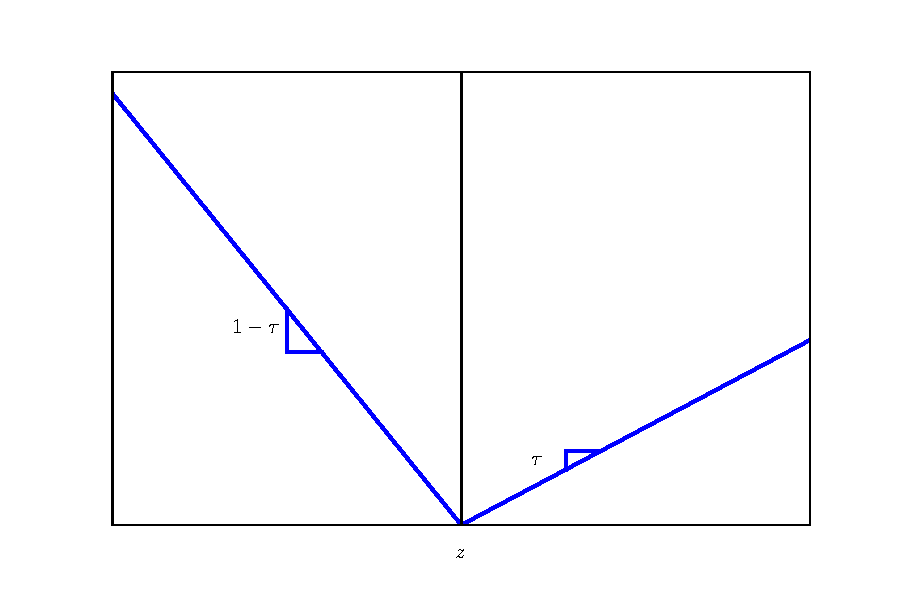
\includegraphics[width = \linewidth]{figures/rho}
\caption*{Notice how $\rho$ "weights" observations on either side of $z=0$ differently. This weighting ensures the propper result from the optimization problem.}
\end{figure}

Quantiles can also be defined as solutions to a minimization problem, specifically by defining $\rho(\cdot)$ as
\begin{equation}
\rho(z) = (\tau - \mathds{1}_{z<0}) \cdot z
\end{equation}
minimizing the expectation of $\rho(y_i - \mu_{\tau})$ will produce the $\tau^{\textrm{th}}$ quantile. Empirically we replace the expectation with a sum, and thus end up with the following estimator for $\hat{\mu}_{\tau}$
\begin{equation}
\hat{\mu}_{\tau} = \underset{\mu_{\tau} \in \mathbb{R}}{\textrm{arg min }} \sum_{i = 1}^N \rho(y_i - \mu_{\tau})
\end{equation}
Of course we're generally not interested in estimating constants. The mosst commonly used approach is to estimate conditional quantiles, whereby the value of $\mu$ depends on $x$ and parameters $\theta$, which are then the goal of optimization. In other words one normally solves
\begin{equation}
\hat{\theta}_{\tau} = \underset{\theta_{\tau} \in \mathbb{R}}{\textrm{arg min }} \sum_{i = 1}^N \rho(y_i - \mu(x_i, \theta_{\tau}))
\end{equation}
The lecture slides covers a heteroscedasticity model, as well as an example of quantile regression applied to birth weight. These are left out here. 
